\documentclass[13pt]{article}
\usepackage[utf8]{inputenc}
\usepackage{polski}
\usepackage{amsmath}%matma
\usepackage{graphicx}%zdjecia
\usepackage{siunitx}
\usepackage{a4wide}
\graphicspath{{./figures/}}
\usepackage[framemethod=TikZ]{mdframed}

\newcommand{\definebox}[2]{%
  \newcounter{#1}
  \newenvironment{#1}[1][]{%
    \stepcounter{#1}%
    \mdfsetup{%
        frametitle={%
            \tikz[baseline=(current bounding box.east),outer sep=0pt]
            \node[anchor=east,rectangle,fill=white]
            {\strut \MakeUppercase#1~\csname the#1\endcsname\ifstrempty{##1}{}{:~##1}};}}%
    \mdfsetup{innertopmargin=1pt,linecolor=#2,%
        linewidth=2pt,topline=true,
        frametitleaboveskip=\dimexpr-\ht\strutbox\relax,}%
    \begin{mdframed}[]\relax%
    }{\end{mdframed}}%
}

\definebox{definition}{black!60}

\title{Nakładanie warstw niskociśnieniową metodą Cold Spray}
\author{Mikołaj Małecki 237339 K00-24b}
\begin{document}
	\maketitle
\section{Wprowadzenie}
Metoda cold spray to metoda addytywnego wytwarzania powłok bądź całych elementów. Polega ona na wyrzucie materiału nanoszonego w postaci drobnego ($5-150 [\si{\micro}m]$) stałego proszku wraz z gazem nośnym (np. tlen, hel). Gaz z doprowadzanym proszkiem jest wystrzeliwany z dużą prędkością rzędu do $1200\frac{m}{s}$. Proszek uderzający o powierzchnie materiału odkształca się plastycznie i generuje niewielką ilość energii cieplnej.

\begin{figure}[!h]
	\centering
	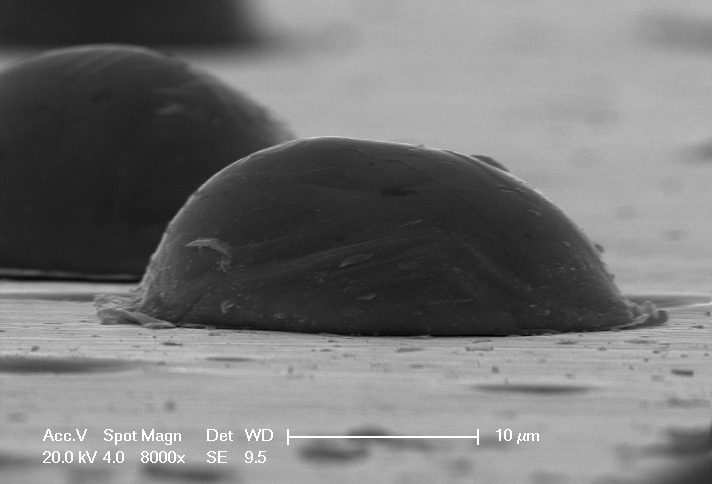
\includegraphics[width=0.3\textwidth]{surf.jpeg}
	\caption{Zdjęcie drobinki tytanu natryskanego na powierzchnię stali \cite{wiki}}
\end{figure}

Z uwagi na naturę tej metody - nie jest ona szczególnie dokładna, natomiast wykorzystuje się ją do technik produkcji przyrostowej metali, polimerów, ceramik czy kompozytów. Element wytworzony lub uzdatniony tą metodą oczywiście trzeba poddać obróbce wykańczającej, natomiast i tak umożliwia wiele dodatkowych przypadków użycia w porównaniu do obróbki ubytkowej. Jednym z takich przypadków jest "drukowanie" 3D metodą cold spray do której nawiązanie można będzie znaleźć w późniejszej sekcji dokumentu.

\begin{figure}[!h]
	\centering
	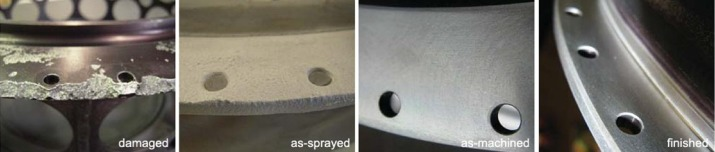
\includegraphics[width=\textwidth]{bef.jpg}
	\caption{Proces renowacji \cite{additive}}
\end{figure}

\newpage

\section{Technika metody}
Technikę natryskiwania na zimno można podzielić na dwie kategorie:
\begin{itemize}
\item wysoko ciśnieniową $>1MPa$
\item nisko ciśnieniową $<1MPa$
\end{itemize}
Różnią się miejscem podawania materiału natryskiwanego oraz w wysokociśnieniowej metodzie gaz pod ciśnieniem jest rozdzielany na dwa strumienie jak na rysunku poniżej:

\begin{figure}[!h]
	\centering
	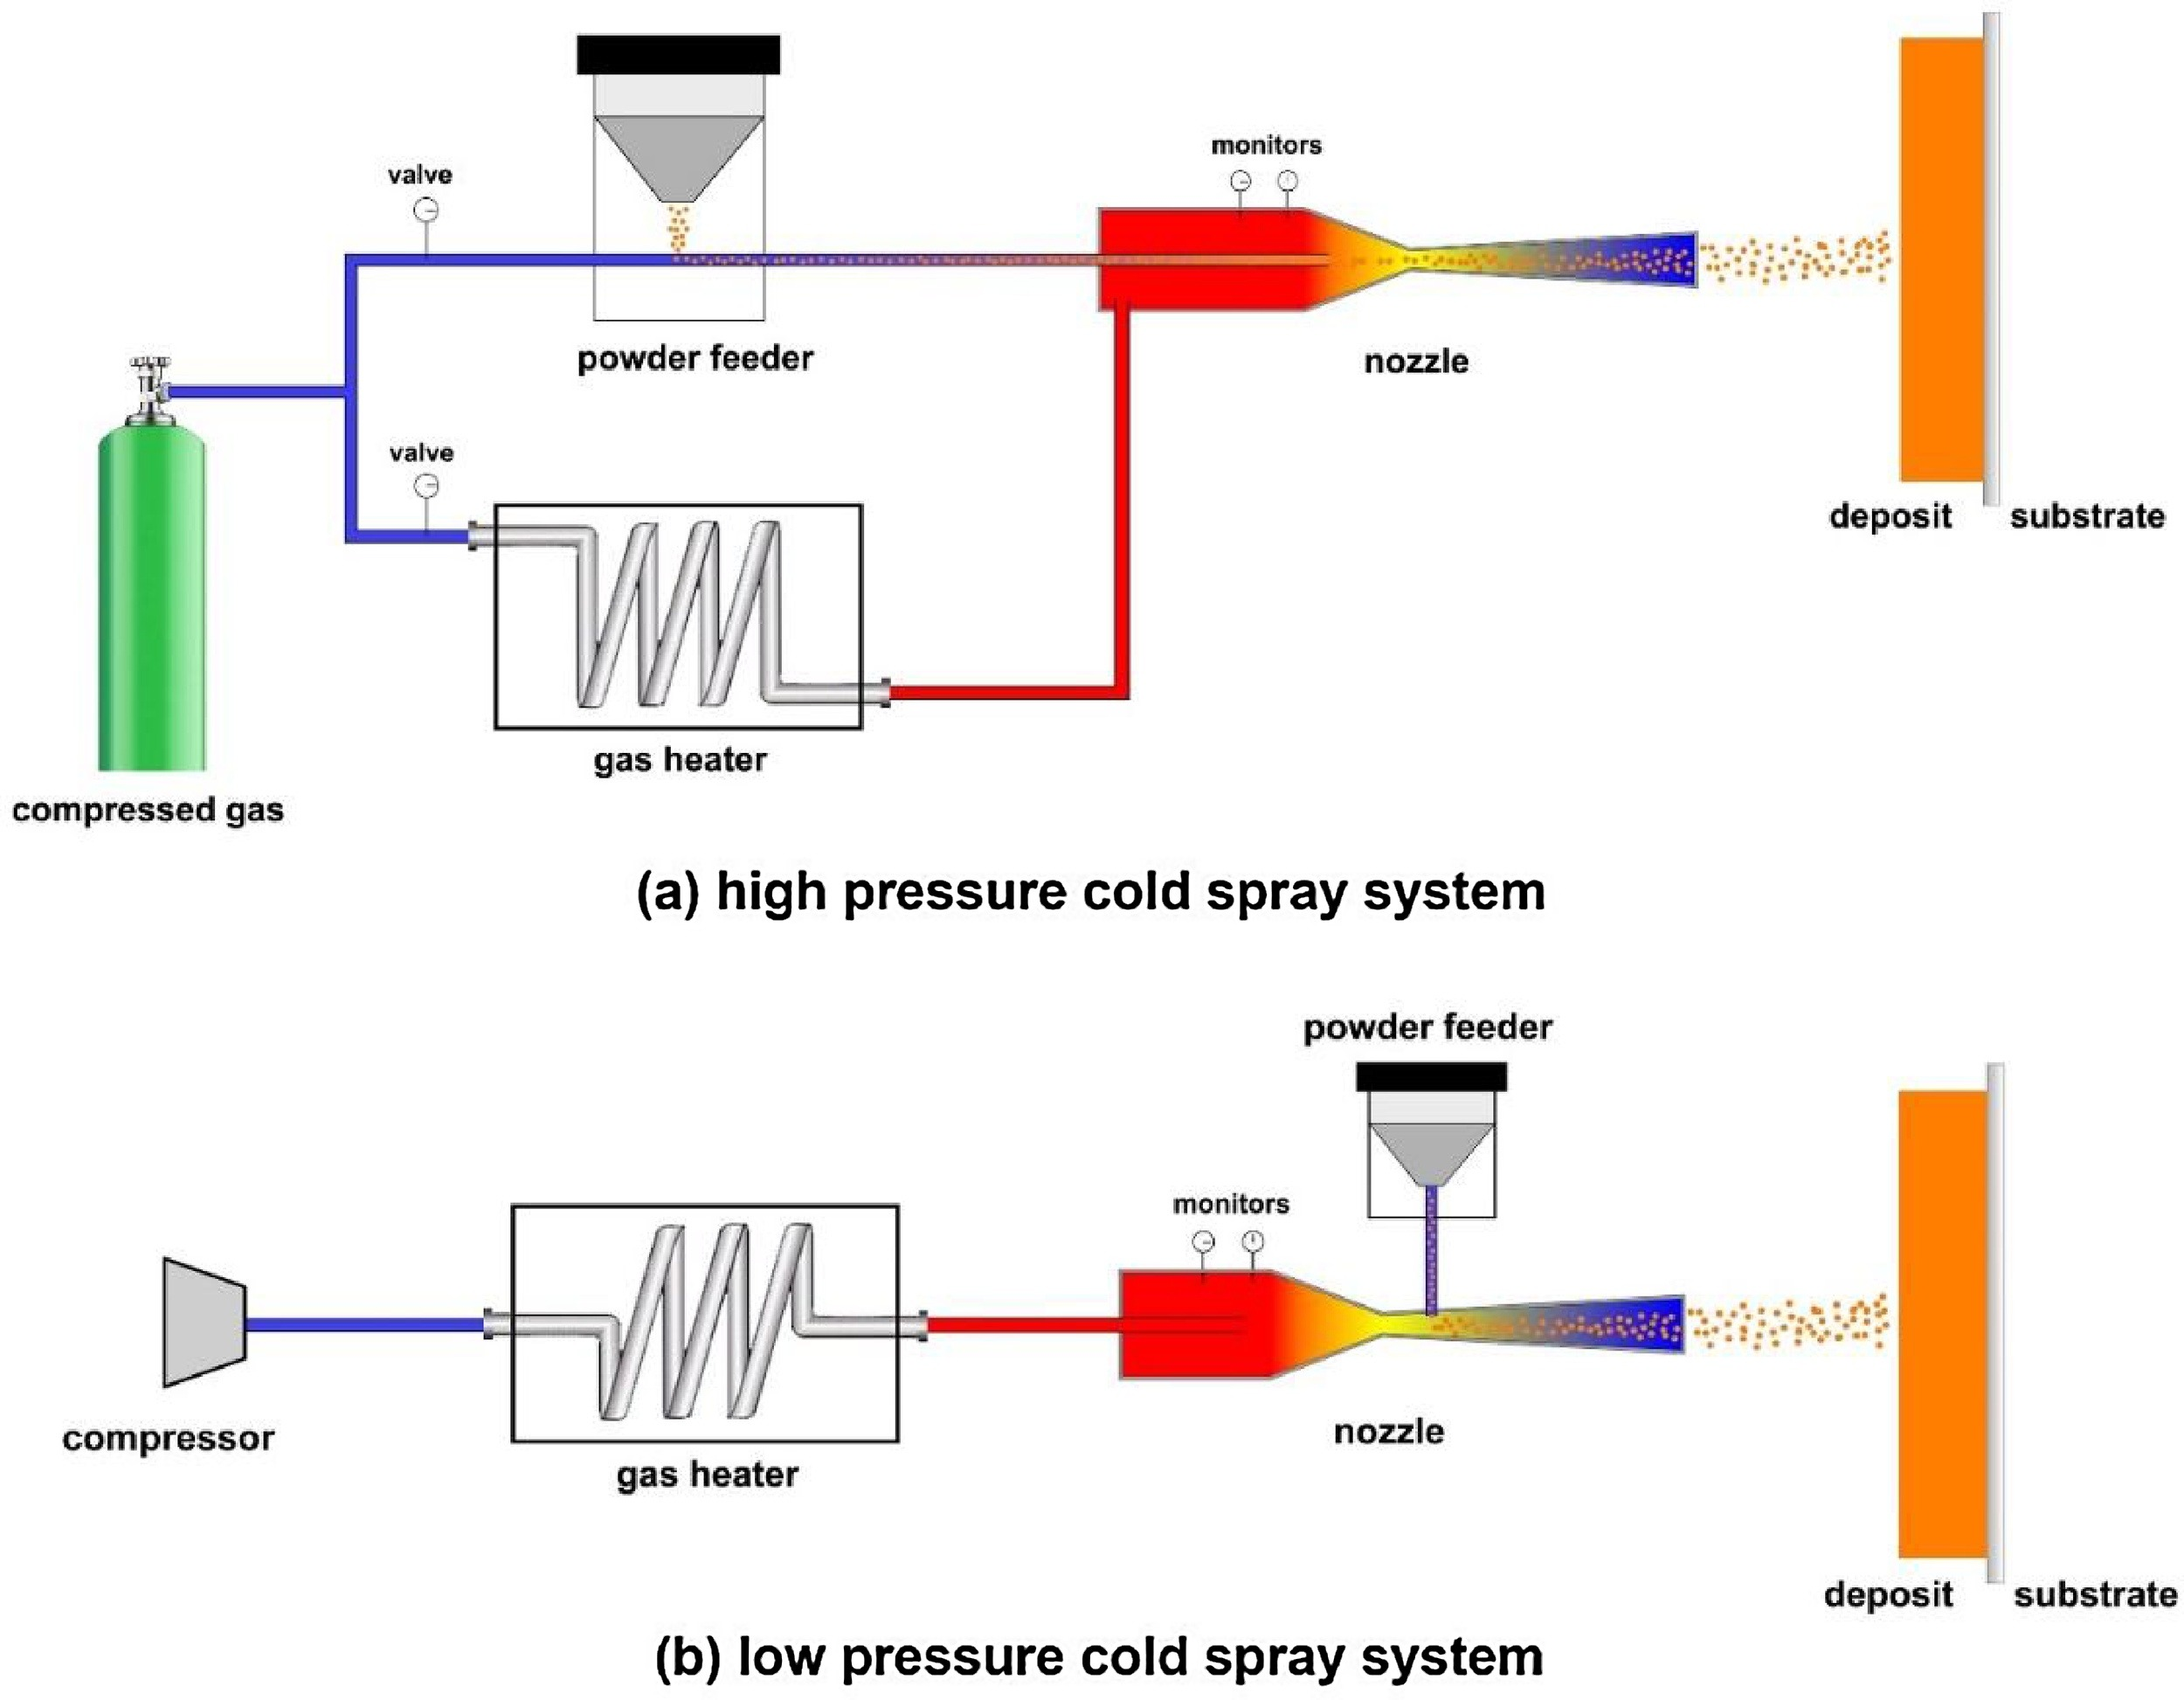
\includegraphics[width=0.8\textwidth]{sys.jpg}
	\caption{ Schemat systemów natrysku zimnym gazem \cite{additive}}
\end{figure}

Ważnym elementem tego systemu jest Dysza de Lavala:
\begin{definition}[Dysza de Lavala]
Kanał aerodynamiczny dzięki któremu można uzyskać przepływ naddźwiękowy wykorzystywany w niektórych typach turbin parowych, w silnikach odrzutowych i rakietowych. Wynalazcą urządzenia jest Gustaf de Laval (1845–1913), szwedzki inżynier i przemysłowiec. \cite{wikil}
\end{definition}

Materiał nanoszony musi uzyskiwać wysokie wartości prędkości wyrzutu żeby na kontrolowanej odległości od płaszczyzny nanoszenia uzyskiwać żadane parametry warstwy.

\newpage

\section{Technika addytywna}
Druk 3D z użyciem cold spray'u ma dużo mniejszy zakres zastosowań niż tradycyjny druk 3D FDM czy SLA, jest to spowodowane mniejszą dokładnością nanoszenia z uwagi na szeroki rozrzut cząsteczek nanoszonego materiału podczas kontatku z powierzchnią. Najlepsze efekty dla tej metody uzyskuje się dla brył obrotowych gdzie układ współżędnych zamiast kartezjańskiego jest biegunowy. Rozrzut natryskiwanych cząsteczek wyrównuje się na kolejnych warstwach dla całego elementu.

\section{Podsumowanie}
Technika ta świetnie nadaje się do nanoszenia warstw ochronnych oraz reperowania zużytych powierzchni lub nawet części elementów. Jednakże z uwagi na niedeterministyczną naturę procesu jego zastosowanie w produkcji precyzyjnych elemntów zostanie tylko mrzonką pasjonatów tradycyjnego druku 3D.

\begin{figure}[!h]
	\centering
	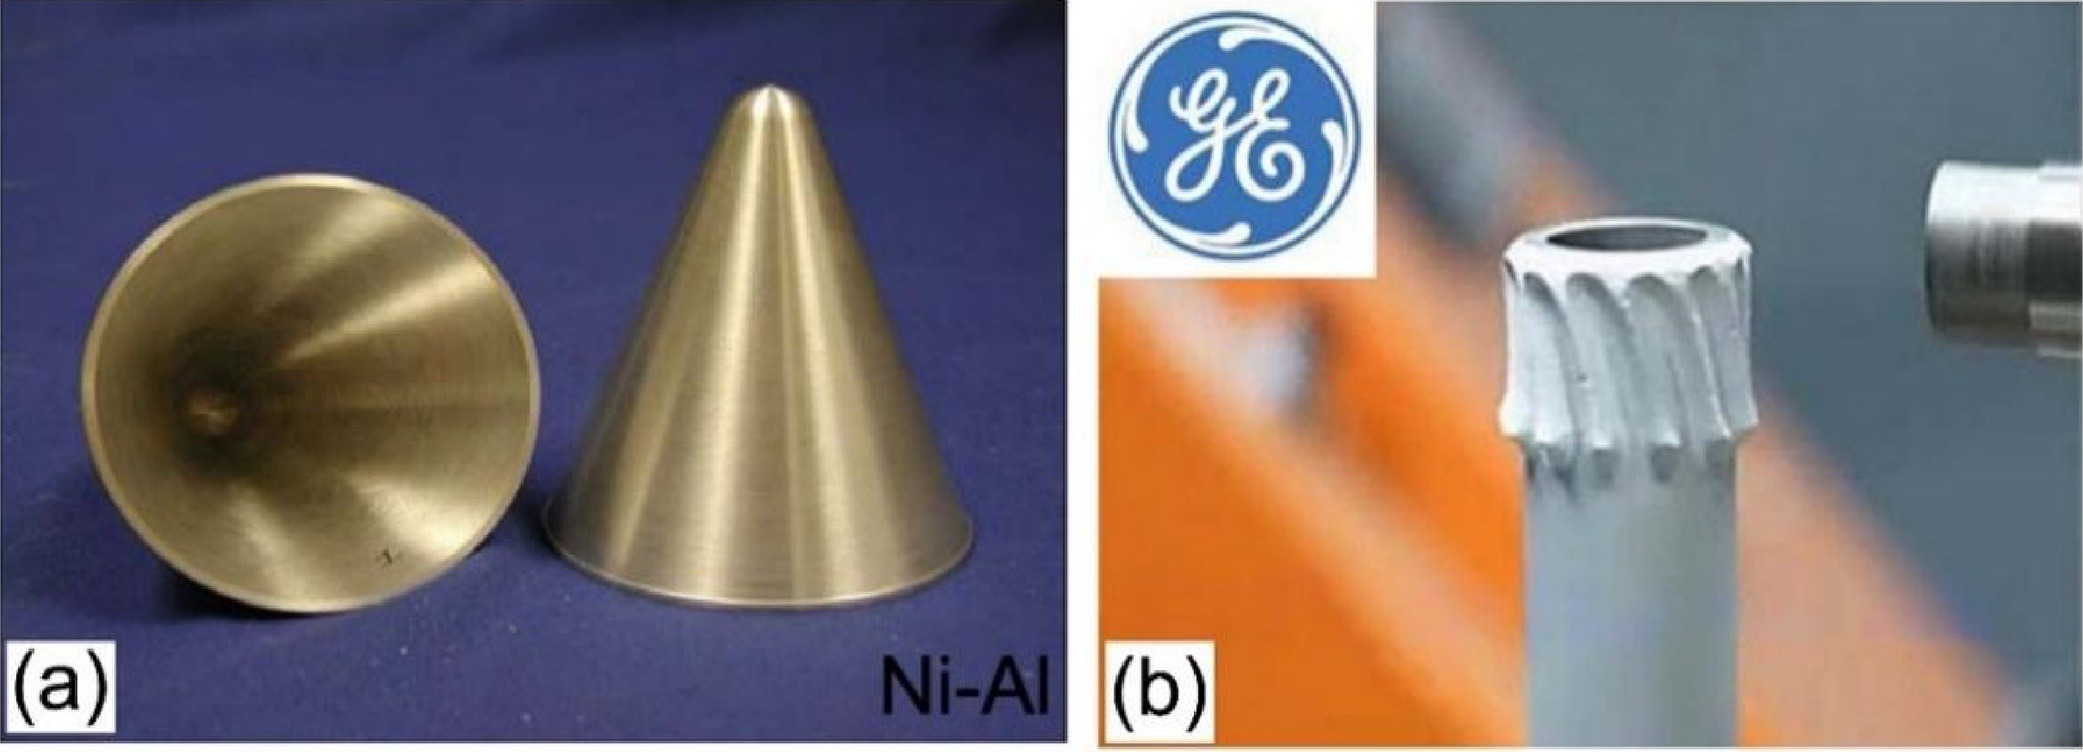
\includegraphics[width=0.8\textwidth]{res.jpg}
	\caption{ Elementy o złożonym kształcie wykonane metodą druku 3D cold spray \cite{additive}}
\end{figure}
\begin{thebibliography}{9}
\bibitem{additive} 
Shuo Yin
\textit{Additive Manufacturing}. 
\\\texttt{https://www.sciencedirect.com/science/article/pii/S2214860417302993}


\bibitem{wiki} 
From Wikipedia, the free encyclopedia
\textit{Cold spraying}. 
\\\texttt{https://en.wikipedia.org/wiki/Cold\_spraying}

\bibitem{wikil} 
From Wikipedia, the free encyclopedia
\textit{Dysza de Lavala}. 
\\\texttt{https://pl.wikipedia.org/wiki/Dysza\_de\_Lavala}
\end{thebibliography}
\end{document}

